\vspace*{10pt}
\begin{center}
    \huge{\textbf{
    \textit{Those who cannot remember the past\\ are condemned to repeat it.}}}
    \large{- George Santayana \autocite{history-quoteSantayana}}
    Wer seine Geschichte nicht kennt, ist dazu verdammt, sie zu wiederholen.\\
    - Freie Übersetzung -
\end{center}
\vspace*{40pt}
\begin{figure}[h]
    \centering
    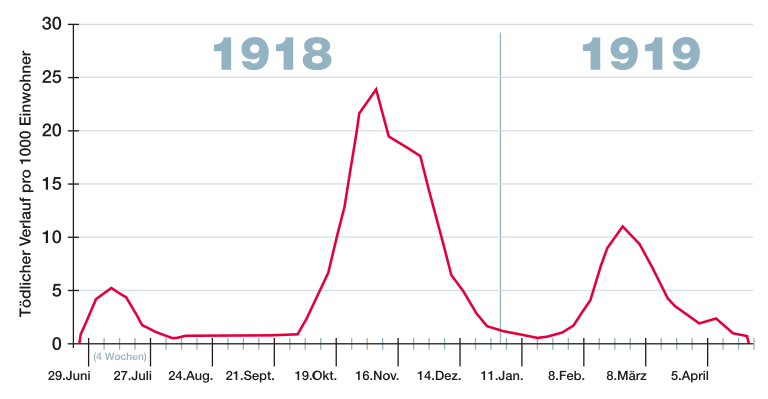
\includegraphics[width=0.72\textwidth]{figures/vor_dem_Inhaltsverzeichniss/Spanische_Grippe_1918_1919_GB.svg.png}
    \caption{Die drei Wellen der \glqq{}Spanischen Grippe\grqq{} in Großbritannien, wöchentliche kombinierte Grippe- und Lungenentzündungssterblichkeit von Juni 1918 bis Mai 1919. \autocite{spanischflu}}
    \label{fig:spanishflu}
\end{figure}
\vspace*{11pt}
\begin{figure}[h]
    \centering
    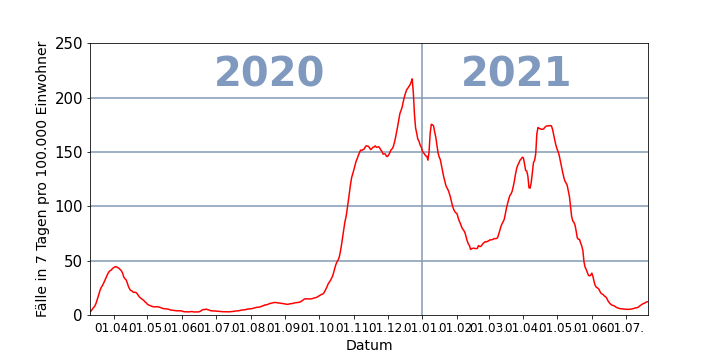
\includegraphics[width=0.75\textwidth]{figures/vor_dem_Inhaltsverzeichniss/Inzidenz_Deutschland.png}
    \caption{Die drei Wellen der COVID-19-Pandemie in Deutschland, dargestellt durch die sieben Tage Inzidenz jeden Tages vom 01.03.2020 bis 21.07.2021. Aus den Daten des Robert-Koch-Instituts erstellt.}
    \label{fig:germany_incidence}
\end{figure}